\documentclass[journal]{IEEEtran}
\usepackage{amsmath,amssymb,booktabs,cite,graphicx}
\usepackage{flushend}
\usepackage{tikz}
\usetikzlibrary{arrows.meta,positioning,calc}
\usepackage[hidelinks]{hyperref}
\newtheorem{proposition}{Proposition}
\newtheorem{theorem}{Theorem}
\newtheorem{corollary}{Corollary}
\newcommand{\E}{\mathbb E}
\newcommand{\KLb}{D_{\mathrm{KL},2}}
\newcommand{\Sep}{\mathcal S_{\rm sep}}
\DeclareMathOperator{\Cov}{Cov}
\DeclareMathOperator{\rank}{rank}
\title{When Does a Learned Coding Surface Change a Semantic Encoder?}
\author{} % Supply the confirmed byline at submission.
\begin{document}
\maketitle
\begin{abstract}
A semantic encoder that assigns observations to shared reconstruction anchors can be changed by reshaping its coding surface or by reweighting the anchors. We separate the two effects when every method is scored by one fixed task distortion. For finite Gibbs encoders, a cost change is absorbed by anchor masses exactly when its two-by-two cross differences vanish. The excess of the rate--distortion Lagrangian over the Blahut optimum is a divergence between encoders, and suitable masses keep it below $\epsilon^2/(2\ln2)$ bits, where $\epsilon$ is the largest non-absorbable logit residual. A $d$-dimensional surface with dot-product logits reproduces the optimal encoder if and only if the doubly centered evaluation cost has rank at most $d$, and a single Euclidean surface does so only for costs of negative type. On a nonuniform 96-state circle at squared-arc distortion 0.30, mass optimization on the intrinsic cost attains the optimal 1.1832 bits per state, the best single Euclidean chord surface needs 1.1899, and spectral dot-product surfaces of dimension 16 and 32 need 1.1837 and 1.1833. Paired measurements on frozen image representations show a nonzero residual at one operating point.
\end{abstract}
\begin{IEEEkeywords}
Semantic communication, rate--distortion theory, Blahut--Arimoto algorithm, metric learning, softmax bottleneck.
\end{IEEEkeywords}

\section{Introduction}
\IEEEPARstart{T}{ask}-oriented transmitters map a learned representation to a finite set of receiver actions and are trained end to end \cite{xie2021deepsc,gunduz2023beyond}. A dense region of the learned surface may attract more probability because anchors are closer, because they carry larger prior masses, or both. Distortion measured in the updated coordinates compounds the ambiguity, since a contraction lowers the measured loss with identical decoded objects. We therefore fix the evaluation cost and ask which geometric changes produce assignments that mass changes cannot.

Indirect and goal-oriented rate--distortion theory turns a latent semantic criterion into a cost on the observable source \cite{liu2022indirect,stavrou}, with shared side information entering as a conditional problem \cite{Guo_2026}. For a finite cost matrix, the Blahut iteration and its semantic extension optimize the reproduction mass \cite{blahut1972computation,csiszar1974,Han_2025}, which also underlies empirical bounds \cite{yang_sandwich,yang_wgd}. Geometry enters through quantizer point density \cite{iacobelli2016quantization}, pulled-back information metrics and the geometry of softmax heads \cite{arvanitidis2022pullinginformationgeometry,park2026informationgeometrysoftmaxprobing}, and isometric or low-bending embeddings \cite{kato,braunsmann}. These works do not identify what a learned surface adds once the masses are free. The contributions of this letter are as follows.
\begin{itemize}
\item An exact criterion separating mass from geometry, a scalar residual that measures it, and the first variation of the constrained objective.
\item An identity for the excess over the Blahut optimum, which bounds the gain of any surface by the squared interaction residual.
\item The interaction rank of an evaluation cost. It equals the smallest surface dimension that realizes the optimal encoder, and a negative-type condition governs a single shared Euclidean surface.
\item A matched-distortion study of four encoder families and spectral surfaces, and paired measurements on frozen image features with a transmitted index.
\end{itemize}

\section{System Model and Problem Formulation}
\subsection{Semantic source and fixed evaluator}
A sensor observes $X$. The context $C$ holds the task index and all knowledge shared before transmission, including the task head and the anchors. A frozen reference encoder gives the unit feature $U=E_0(X,C)$, and $q(u)=P(Y=\cdot\mid U=u,C)$ is the posterior of the task variable $Y$. Under log loss the indirect problem reduces to a cost on $U$ \cite{liu2022indirect}, and replacing $u$ by $u'$ costs $D_{\rm KL}(q(u)\Vert q(u'))=\tfrac12 v^\top J_q^\top{\rm diag}(1/q)J_q v+o(\|v\|^2)$ for $v=u'-u$. This Fisher pullback \cite{arvanitidis2022pullinginformationgeometry} is degenerate along directions that leave the posterior unchanged. We add $\eta g_0$, with $g_0$ the unit-feature metric and $\eta>0$, and realize the sum by the lift $z(u)=(2\sqrt{q(u)},\sqrt{\eta}\,u)$, whose squared chord agrees with the regularized metric to second order.

The finite study has states $z_i$ with probabilities $p_i>0$, $i\le n$, and $M$ shared anchors $\bar z_j$. The evaluation cost $C^g_{ij}\ge0$ is fixed on actual pairs, as $\|z_i-\bar z_j\|^2$ or a squared intrinsic distance. For squared intrinsic distance on a compact boundaryless $m$-manifold with smooth positive density, the rate--distortion function has leading term $h_g(p)-(m/2)\ln(2\pi eD/m)$ nats \cite{linder1999high}. Expanding the volume element adds $D\,\E[\mathrm{Scal}_g]/(6m)$ under uniform remainder conditions, which is $D/6$ on the unit two-sphere, whereas ambient chord loss brings in the second fundamental form. The training criterion is thus part of the benchmark. Transporting source, alphabet and cost through a bijection preserves the function. A learned chart can therefore help only a restricted interface, as specified next and shown in Fig.~\ref{fig:system}.


\subsection{Encoder family, payload and link}
\begin{figure}[t]\centering
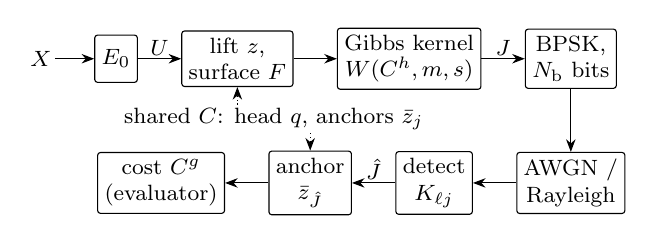
\begin{tikzpicture}[font=\footnotesize,>={Stealth[length=1.6mm]},
 blk/.style={draw,rounded corners=1pt,minimum height=6mm,inner sep=2.5pt,align=center}]
\node[blk] (e0) {$E_0$};
\node[blk,right=5.5mm of e0] (f) {lift $z$,\\surface $F$};
\node[blk,right=5.5mm of f] (w) {Gibbs kernel\\$W(C^h,m,s)$};
\node[blk,right=5.5mm of w] (tx) {BPSK,\\$N_{\rm b}$ bits};
\node[blk,below=8mm of tx] (ch) {AWGN /\\Rayleigh};
\node[blk,left=5.5mm of ch] (det) {detect\\$K_{\ell j}$};
\node[blk,left=5.5mm of det] (look) {anchor\\$\bar z_{\hat J}$};
\node[blk,left=5.5mm of look] (ev) {cost $C^g$\\(evaluator)};
\node[inner sep=1pt] (ctx) at ($(f.south)!0.5!(look.north)$) {shared $C$: head $q$, anchors $\bar z_j$};
\draw[->] ([xshift=-5mm]e0.west) node[left,inner sep=1pt]{$X$} -- (e0);
\draw[->] (e0) -- node[above,inner sep=1pt]{$U$} (f);
\draw[->] (f) -- (w);
\draw[->] (w) -- node[above,inner sep=1pt]{$J$} (tx);
\draw[->] (tx) -- (ch);
\draw[->] (ch) -- (det);
\draw[->] (det) -- node[above,inner sep=1pt]{$\hat J$} (look);
\draw[->] (look) -- (ev);
\draw[->,densely dotted] (ctx.north-|f) -- (f.south);
\draw[->,densely dotted] (ctx.south-|look) -- (look.north);
\end{tikzpicture}
\caption{Finite semantic interface. Only the index $J$ crosses the link. The evaluator is common to all encoders and is never retrained.}
\label{fig:system}\end{figure}
A stochastic encoder $W_{ij}=\Pr(J=j\mid i)$ has output marginal $\bar W_j=\sum_i p_iW_{ij}$ and
\begin{align}
 I_2(W)&=\sum_{ij}p_iW_{ij}\log_2(W_{ij}/\bar W_j),\nonumber\\
 D_g(W)&=\sum_{ij}p_i W_{ij} C^g_{ij}.
\end{align}
The transmitter computes a coding cost $C^h_{ij}=\|F(z_i)-F(\bar z_j)\|^2$ on a surface $F$ and draws $J$ from the Gibbs kernel
\begin{equation}
 W_{ij}(C^h,m,s)=\frac{m_j\exp(-sC^h_{ij})}{\sum_k m_k\exp(-sC^h_{ik})},\label{eq:kernel}
\end{equation}
with scale $s>0$ and masses $m_j>0$. In a quadrature $m_j\propto v_jr_j$ combines a cell volume and a density, which act only through their product. The index uses $N_{\rm b}=\lceil\log_2 M\rceil$ uncoded BPSK symbols over AWGN or coherent block Rayleigh fading. If $K_{\ell j}$ is the probability of detecting $j$ when $\ell$ is sent, the receiver returns $\bar z_{\hat J}$ with expected distortion
\begin{equation}
 D_{\rm rx}=\sum_{i\ell j}p_iW_{i\ell}K_{\ell j}C^g_{ij}.\label{eq:rx}
\end{equation}
For independent bit errors of probability $e$, $K_{\ell j}=e^{d_H(\ell,j)}(1-e)^{N_{\rm b}-d_H(\ell,j)}$. Under block fading this expression is evaluated at the common gain and then averaged. We keep three quantities apart: the test-channel information $I_2(W)$, which long-block source codes can approach, the fixed payload $N_{\rm b}$, and $D_{\rm rx}$.

\subsection{Problem}
For a slope $\lambda>0$ and a penalty weight $\gamma\ge0$ we study
\begin{align}
 \min_{F,m,s}\ & L=I_2(W)+\lambda D_g(W)+\gamma B_{\rm s}(F)\label{eq:objective}\\
 \text{s.t.}\ & (1-\alpha)\|z-v\|\le\|F(z)-F(v)\|\le(1+\alpha)\|z-v\|,\nonumber
\end{align}
with $W$ from \eqref{eq:kernel}, a smoothness penalty $B_{\rm s}$ and $0\le\alpha<1$. Source weights, anchors, evaluator and radio are common to all methods. Four families are compared: fixed surface with uniform masses, learned masses, learned surface, and both. The reference is the finite Blahut value $F(\lambda)=\min_W I_2(W)+\lambda D_g(W)$ over all channels, attained by $W^\star_{ij}\propto\pi^\star_j2^{-\lambda C^g_{ij}}$ with $\pi^\star$ its own output marginal \cite{blahut1972computation}.

\begin{figure*}[t]\centering
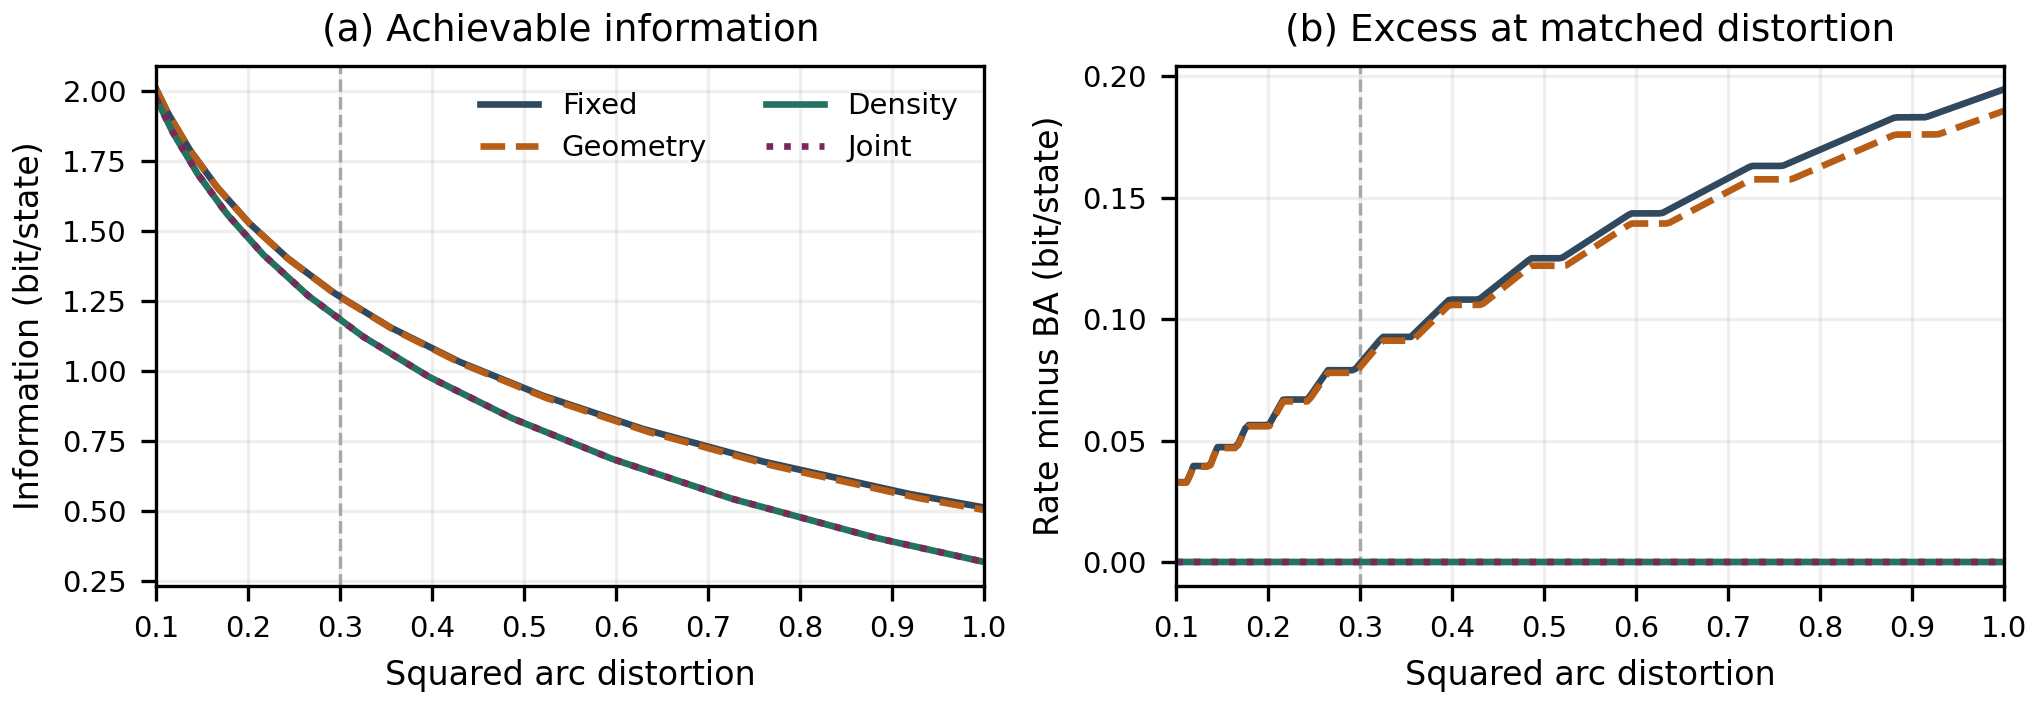
\includegraphics[width=.8\textwidth]{figures/circle_ablation.png}
\caption{Achieved information for the four encoder families on the nonuniform circle (left). Subtracting the finite Blahut curve at the same distortion resolves the contribution of the mass model (right). The dashed vertical line marks the comparison in Table~\ref{tab:circle}.}
\label{fig:ablation}\end{figure*}

\section{Mass, Geometry and Interaction Rank}
Let $\Sep=\{\Delta:\Delta_{ij}=a_i+b_j\}$ be the additively separable $n\times M$ matrices and $H_n=I_n-\mathbf 1\mathbf 1^\top/n$.
\subsection{What mass optimization can absorb}
\begin{proposition}\label{prop:contrast}
Fix $s>0$, a cost $C$ and strictly positive masses $m$. For another cost $C'$ there exist strictly positive $m'$ with $W(C',m',s)=W(C,m,s)$ if and only if $\Delta=C'-C\in\Sep$. Equivalently, for all $i,i',j,k$,
\begin{equation}
 \Delta_{ij}-\Delta_{ik}-\Delta_{i'j}+\Delta_{i'k}=0.\label{eq:contrast}
\end{equation}
\end{proposition}
\begin{IEEEproof}
Equality of the log odds of $j$ against $k$ in row $i$ requires $s(\Delta_{ij}-\Delta_{ik})=\ln(m'_j/m_j)-\ln(m'_k/m_k)$. The right side does not depend on $i$, which gives \eqref{eq:contrast}. Conversely fix $(i_0,k_0)$ and set $a_i=\Delta_{ik_0}$, $b_j=\Delta_{i_0j}-\Delta_{i_0k_0}$. Vanishing contrasts give $\Delta_{ij}=a_i+b_j$. Then $m'_j\propto m_je^{sb_j}$ cancels $b_j$ and row normalization cancels $a_i$.
\end{IEEEproof}
With different scales the test applies to $s'C'-sC$. With zero masses it applies to the common support, and different supports are distinguishable at once. The criterion acts on assignment probabilities and is independent of ambient coordinates. An observable scalar is the root mean square of $H_n(s\Delta)H_M$, in logit units. It vanishes exactly in Proposition~\ref{prop:contrast}. A zero residual means equivalence with unrestricted positive masses, which a low-dimensional mass model may not represent. A nonzero residual shows a change of assignment odds. Its sign does not predict a rate saving.

\subsection{First variation}
Write $A_{ij}=\log_2(W_{ij}/\bar W_j)+\lambda C^g_{ij}$ and $S_{ij}=\delta\ln m_j-s\,\delta C^h_{ij}-C^h_{ij}\delta s$. Row normalization gives $\delta W_{ij}=W_{ij}(S_{ij}-\E_{W_i}S_{ij})$, the constants from the two entropies cancel, and
\begin{equation}
 \delta L=\sum_i p_i\Cov_{W_i}(A_{ij},S_{ij})+\gamma\,\delta B_{\rm s}. \label{eq:variation}
\end{equation}
For squared chords $\delta C^h_{ij}=2\langle F_i-F_j,\delta F_i-\delta F_j\rangle$. For any auxiliary mass $\pi$,
\begin{equation}
 \sum_i p_i\KLb(W_i\Vert\pi)=I_2(W)+\KLb(\bar W\Vert\pi),\label{eq:aux}
\end{equation}
so minibatches train an upper bound through $\pi$ while evaluation uses the full $\bar W$. The auxiliary $\pi$ estimates a marginal and has a different role from the encoder mass $m$.

\subsection{Distance from the Blahut optimum}
\begin{proposition}\label{prop:excess}
Let $(W^\star,\pi^\star)$ attain $F(\lambda)$ and let $V$ be a channel supported on the support of $\pi^\star$. Then
\begin{equation}
 L(V)-F(\lambda)=\sum_i p_i\KLb(V_i\Vert W^\star_i)-\KLb(\bar V\Vert\pi^\star),\label{eq:excess}
\end{equation}
where $L=I_2+\lambda D_g$. If $sC^h-\lambda\ln2\,C^g=a_i+b_j+E_{ij}$ with $|E_{ij}|\le\epsilon$, the masses $m_j\propto\pi^\star_je^{b_j}$ give
\begin{equation}
 L\big(W(C^h,m,s)\big)-F(\lambda)\le\frac{\epsilon^2}{2\ln2}\ \text{bits}.\label{eq:eps}
\end{equation}
\end{proposition}
\begin{IEEEproof}
With $Z_i=\sum_j\pi^\star_j2^{-\lambda C^g_{ij}}$, $\KLb(V_i\Vert\pi^\star)+\lambda\sum_jV_{ij}C^g_{ij}=\KLb(V_i\Vert W^\star_i)-\log_2Z_i$ and $F(\lambda)=-\sum_ip_i\log_2Z_i$. Averaging over $i$ and applying \eqref{eq:aux} with $\pi=\pi^\star$ proves \eqref{eq:excess}. For the second claim, the chosen masses give $V_{ij}\propto W^\star_{ij}e^{-E_{ij}}$. This is an exponential tilt of $W^\star_i$ by a function of range at most $2\epsilon$, whose divergence is at most $(2\epsilon)^2/8$ nats because the variance of the tilting function never exceeds $\epsilon^2$.
\end{IEEEproof}
Taking $\epsilon$ as the smallest sup-norm distance from $sC^h-\lambda\ln2\,C^g$ to $\Sep$, and minimizing over $s$, bounds how far mass optimization on $C^h$ is from optimal. No surface beats $F(\lambda)$, so this also bounds the gain of any reshaping over mass-only training on the same surface. In particular, $C^h=C^g$ and $s=\lambda\ln2$ give $\epsilon=0$, and optimal masses realize the Blahut optimum. A credible geometric gain therefore needs a declared restriction such as a surface dimension, a mass model, a fixed scale or reuse across tasks. The first term of \eqref{eq:excess} weights the residual by the encoder itself and is much sharper than \eqref{eq:eps} when large residuals fall on improbable pairs.

\subsection{Interaction rank}
Dot-product heads compute logits $\langle x_i,y_j\rangle+\beta_j$ from $d$-dimensional embeddings. Up to row and column terms this is the bilinear cost $C^h_{ij}=\|x_i-y_j\|^2$, where states and anchors may use different maps. Let $T=H_nC^gH_M$ and call $r_{\rm int}=\rank T$ the \emph{interaction rank} of the evaluator.
\begin{theorem}\label{thm:rank}
Let $W^\star$ attain $F(\lambda)$ with $\pi^\star>0$. The family $\{W(C^h,m,s)\}$ of bilinear costs in $\mathbb R^d$ contains $W^\star$ if and only if $r_{\rm int}\le d$. If $\pi^\star$ has zero entries, the statement holds with $C^g$ restricted to the supported columns and masses on that support.
\end{theorem}
\begin{IEEEproof}
$W^\star=W(C^g,\pi^\star,\lambda\ln2)$ is a Gibbs kernel. By Proposition~\ref{prop:contrast} applied to the scaled costs, $W(C^h,m,s)=W^\star$ for some $m$ if and only if $sC^h-\lambda\ln2\,C^g\in\Sep$. Since $\|x_i\|^2+\|y_j\|^2\in\Sep$ and double centering annihilates exactly $\Sep$, the condition is $-2sH_nXY^\top H_M=\lambda\ln2\,T$, whose left side has rank at most $d$. Conversely factor $T=UV^\top$ with $d$ columns and set $X=-(\lambda\ln2/(2s))U$, $Y=V$. Then $H_nXY^\top H_M=-(\lambda\ln2/(2s))T$ because $T$ is already doubly centered.
\end{IEEEproof}
One embedding serves all slopes when $s\propto\lambda$. The obstruction is of the softmax-bottleneck type \cite{yang2018breaking}: $\ln W$ has rank at most $d+2$ in the family. Here it is applied to the optimal test channel, and it is measured by a property of the evaluator alone. If $C^g$ is itself a squared distance between points of $\mathbb R^{d_0}$, then $r_{\rm int}\le d_0$.

\begin{corollary}\label{cor:single}
Let states and anchors be the same $n$ points with one map, $C^h_{ij}=\|F_i-F_j\|^2$, and let $C^g$ be symmetric with zero diagonal and $\pi^\star>0$. Some surface in $\mathbb R^d$ realizes $W^\star$ if and only if $-H_nC^gH_n$ is positive semidefinite of rank at most $d$.
\end{corollary}
\begin{IEEEproof}
The matrix $sC^h-\lambda\ln2\,C^g=a_i+b_j$ is symmetric with zero diagonal. Hence $a_i+b_i=0$ and $a_i-b_i$ is constant, so $a_i+b_j=0$. Thus $(\lambda\ln2/s)C^g$ must be a Euclidean squared-distance matrix, which is Schoenberg's condition \cite{schoenberg1935}.
\end{IEEEproof}
Squared arc length on a circle has Fourier coefficients $4(-1)^k/k^2$ of alternating sign, so it is not of negative type. No single Euclidean surface of any dimension reproduces its optimal encoder, whereas a bilinear surface does so at $d=r_{\rm int}$ and approximately below it. A non-iterative baseline keeps the $d$ leading singular triplets of $T$. Its residual has entries at most $\sigma_{d+1}(T)$ \cite{eckart1936}, so by \eqref{eq:eps} its excess is at most $(\lambda\ln2\,\sigma_{d+1}(T))^2/(2\ln2)$ bits.

These statements suggest a three-step diagnosis before training a surface. First, the singular values of $T$ show which surface dimensions can matter for the declared evaluator. Second, the doubly centered residual of a candidate coding cost tests whether it differs from the reference beyond a mass change. Third, a sweep of slopes compares rates at equal $D_g$, since neither a nonzero residual nor a lower Lagrangian at one slope establishes a saving.

\section{Implementation and Results}
\subsection{Bounded learned surface}
With $z$ the lift of Section~II and $C^g_{ij}=\|z_i-\bar z_j\|^2$, the learned surface is
\begin{equation}
 F(z)=z+\alpha B_1\tanh(A_1z),\qquad 0\le\alpha<1 ,
\end{equation}
with the Frobenius norms of $A_1,B_1$ clipped to one. The perturbation is $\alpha$-Lipschitz, which enforces the constraint in \eqref{eq:objective} on new inputs as well as on training points and excludes collapse. The penalty $B_{\rm s}$ is the sample mean of $\|F(z)+F(v)-2F((z+v)/2)\|^2$ for a nearest distinct anchor $v$. The midpoint lives in the ambient space, so the penalty regularizes the extension used by the encoder and does not estimate intrinsic curvature. Training follows \eqref{eq:variation} with the auxiliary mass of \eqref{eq:aux}.

\subsection{A circle on which density explains the rate saving}
On a 96-point circle use $\theta_i=2\pi(i+1/2)/96$, $p_i=(1+0.85\cos\theta_i)/96$ and the same points as anchors. The evaluator is squared shortest arc on the original circle. A positive speed with four Fourier coefficients, normalized to circumference $2\pi$, defines the coding arcs. Eight further coefficients parameterize log density relative to the arc quadrature weights, so geometry-only training also moves the cell volumes. All four families optimize the scale on the same 25 slopes, and a finite Blahut solver on the original cost gives the reference.
\begin{table}[t]
\caption{Rates at fixed squared arc distortion $D_g=0.30$. Values interpolate achievable points on the same 96-state source.}\label{tab:circle}\centering
\begin{tabular}{lc}\toprule Encoder family & Information (bit/state)\\\midrule
Fixed surface and uniform mass & 1.264985\\
Learned surface, density fixed & 1.263440\\
Fixed surface, learned density & 1.183192\\
Learned surface and density & 1.183192\\
Finite Blahut reference & 1.183191\\\bottomrule
\end{tabular}\end{table}
Table~\ref{tab:circle} attributes 0.08179 bit per state of saving to density alone, against 0.00155 for the speed change with fixed density. This is the case $\epsilon=0$ of Proposition~\ref{prop:excess}: the fixed surface carries the evaluation cost, and masses suffice. The joint and density rates differ by less than $10^{-7}$ bit, below the precision of interpolation on the common slope grid. These are rates of stochastic test channels, not fixed-length packet savings. Figure~\ref{fig:ablation} compares interpolants over the shared distortion range, and every abscissa uses squared arc on the unwarped circle. Measuring distortion along the learned arc would move points horizontally as well and confound the comparison.

\begin{table}[t]
\caption{Restricted surfaces on the same circle with optimized masses and scale. Excess and bound are in bits at the grid slope $\lambda\ln2=1.542$ with matched scale and centering masses.}\label{tab:rank}\centering
\begin{tabular}{lccc}\toprule
Coding surface & Rate at $0.30$ & Excess \eqref{eq:excess} & Bound \eqref{eq:eps}\\\midrule
Euclidean chord, $d=2$ & 1.189914 & --- & ---\\
Spectral, $d=2$ & 1.189897 & 0.10346 & 11.40\\
Spectral, $d=4$ & 1.210406 & 0.07020 & 4.262\\
Spectral, $d=8$ & 1.187964 & 0.00860 & 1.325\\
Spectral, $d=16$ & 1.183713 & 0.00074 & 0.360\\
Spectral, $d=32$ & 1.183265 & 0.00006 & 0.082\\\bottomrule
\end{tabular}\end{table}
Table~\ref{tab:rank} restricts the surface instead. The centered squared-arc cost has numerical rank 95 with singular values $192.07, 48.07, 21.40, 12.07,\dots$ in equal pairs, and $-T$ has eigenvalues of both signs. The best unit-circle chord surface with free masses and scale stays 0.0067 bit above the Blahut rate, consistent with Corollary~\ref{cor:single}, which excludes exact optimality for every single Euclidean surface. Spectral surfaces approach the optimum as $d$ grows, as Theorem~\ref{thm:rank} predicts, and the supremum residual of the truncation falls from 2.58 to 0.22. The approach is not monotone: $d=4$ is worse than $d=2$ because the truncated series is flat near zero arc, where the encoder concentrates. The encoder-weighted divergence in \eqref{eq:excess} captures this effect, while the worst-case bound \eqref{eq:eps} becomes informative only once the logit residual is below one. The optimal marginal has full support at this slope.

\subsection{Paired measurements on real feature clouds}
SEMASIA supplies frozen CIFAR-100 representations \cite{semasia}. On ResNet-18 we use the 20-way coarse task, disjoint fitting and calibration IDs, and the same anchors, costs and channel model for all four modes. The code stores the two-layer deformation, masses and head.
\begin{table}[t]
\caption{The same 2,048 official SEMASIA test IDs and 16 anchors. Residual is RMS doubly centered $5(C^h-C^g)$ in logit units.}\label{tab:real}\centering
\begin{tabular}{lrrrr}\toprule
Mode & Residual & $I_2$ & $D_g$ & $I_2+3D_g$\\\midrule
Fixed & 0 & 3.5205 & 1.7805 & 8.8620\\
Density & 0 & 3.5208 & 1.7807 & 8.8630\\
Geometry & 0.2621 & 3.4975 & 1.7859 & 8.8551\\
Joint & 0.2619 & 3.4978 & 1.7862 & 8.8565\\\bottomrule
\end{tabular}\end{table}
Table~\ref{tab:real} evaluates all saved encoders on the same 2,048 official test IDs. At fixed scale $s=5$, geometry changes the row odds beyond what any change of masses can produce. Its information decreases by 0.0230 bit per image relative to the fixed mode, while $D_g$ increases by 0.0054. This single operating point documents a tradeoff, and a gain at equal distortion requires a slope sweep. The last column excludes the training penalty and uses the full-test output marginal. The saved run uses 768 fitting images, 192 calibration images, 16 anchors and two epochs. Its four-bit interface verifies that training, held-out inference and index transmission are connected. Replicated training and matched-distortion sweeps on larger codebooks are needed to compare rate gains across backbones.

\subsection{From the stochastic encoder to a received index}
Equation \eqref{eq:rx} evaluates a trained surface on a physical link, where geometry, masses and bit-to-anchor assignment all affect the received distortion. In a separate link check, the joint checkpoint sent four bits per image on 192 official test IDs, with two noise and index draws. Clean reception gave fixed distortion 1.7921. At $E_b/N_0=0$ dB, AWGN gave 3.1857 with index error 0.3073, and Rayleigh gave 3.5210 with index error 0.3984. At 10 dB the Rayleigh index error fell to 0.0625 and the distortion to 2.0190. These are measurements at a common physical payload. The information figures in Table~\ref{tab:real} describe the stochastic encoder before detection.

\section{Conclusion}
A geometric deformation changes a finite Gibbs encoder beyond mass reweighting exactly when it changes a cross difference of coding costs, and its possible benefit in the rate--distortion Lagrangian is bounded by the squared interaction residual between coding logits and the evaluation cost. The interaction rank of the evaluator gives the surface dimension at which a dot-product encoder becomes optimal, and negative type decides whether one shared Euclidean surface can be. On the circle, density on the intrinsic cost is already optimal and low-dimensional surfaces pay a measurable rate. Whether geometry saves rate on real feature clouds remains to be settled by matched-distortion sweeps.
\bibliographystyle{IEEEtran}
\bibliography{ref}
\end{document}
